\documentclass[conference]{IEEEtran}
\IEEEoverridecommandlockouts
\usepackage{cite}
\usepackage{amsmath,amssymb,amsfonts}
\usepackage{graphicx}
\usepackage{textcomp}
\usepackage{xcolor}
\usepackage{booktabs}
\usepackage{array}
\usepackage{url}
\usepackage{hyperref}

% Auto-generated macros for NASA FIRMS VIIRS Disturbance Pipeline
\newcommand{\numDetections}{2,299}
\newcommand{\numTrainDetections}{1,609}
\newcommand{\numTestDetections}{690}
\newcommand{\dateMin}{2026-10-17}
\newcommand{\dateMax}{2026-10-21}
\newcommand{\numSaturatedPixels}{43}
\newcommand{\numSpatialTiles}{464}
\newcommand{\accDummy}{34.8}
\newcommand{\accCoords}{99.8}
\newcommand{\accGeomOnly}{53.0}
\newcommand{\accTiFiveOnly}{52.3}
\newcommand{\accLogReg}{55.4}
\newcommand{\accDt}{61.6}
\newcommand{\accMlp}{61.7}
\newcommand{\accRf}{63.1}
\newcommand{\accHgb}{60.3}
\newcommand{\accSwathGeom}{83.4}
\newcommand{\shortcutBoost}{23.1}
\newcommand{\accSpatialBlockCv}{55.5}
\newcommand{\accSpatialBlockCvStd}{5.8}
\newcommand{\spatialLeakageInflation}{4.8}
\newcommand{\fOneDummy}{10.3}
\newcommand{\fOneLogReg}{54.4}
\newcommand{\fOneDt}{57.0}
\newcommand{\fOneMlp}{57.8}
\newcommand{\fOneRf}{60.4}
\newcommand{\fOneHgb}{58.5}
\newcommand{\fOneGeomOnly}{47.3}
\newcommand{\fOneSwathGeom}{81.3}
\newcommand{\recHgb}{58.2}
\newcommand{\topFeature}{bright_ti5}
\newcommand{\featImpTiFive}{36.6}
\newcommand{\featImpDeltaT}{16.9}
\newcommand{\featImpTiFour}{14.6}
\newcommand{\featImpLogFrp}{13.8}
\newcommand{\featImpFrp}{13.4}
\newcommand{\featImpDaytime}{4.6}
\newcommand{\recBorealHgb}{83.1}
\newcommand{\recPeatlandHgb}{70.8}
\newcommand{\recFlaringHgb}{63.8}
\newcommand{\precFlaringHgb}{66.7}
\newcommand{\flaringDeltaTMed}{20.5}
\newcommand{\flaringTiFourMed}{300.3}
\newcommand{\flaringFrpMed}{0.85}
\newcommand{\borealDeltaTMed}{51.6}
\newcommand{\borealTiFiveMed}{277.9}


\begin{document}

\title{Satellite Thermal Anomaly and Disturbance Regime Characterization across Global Forest and Agricultural Frontiers}

\author{
\IEEEauthorblockN{Cristhian David Caceres Mateus}
\IEEEauthorblockA{\textit{Department of  Business} \\
\textit{Univ. of Europe for Applied Sciences}\\
Potsdam 14469, Germany \\
cristhian.caceres@ue-germany.de}
\and
\IEEEauthorblockN{Talha Ali Khan}
\IEEEauthorblockA{\textit{Department of  Business} \\
\textit{Univ. of Europe for Applied Sciences}\\
Potsdam 14469, Germany \\
talhaali.khan@ue-germany.de}
}
\maketitle

\begin{abstract}
Rapid characterization of environmental disturbances---distinguishing commodity-driven tropical deforestation from agricultural residue burning, petrochemical gas flaring, boreal wildfires, and peatland clearing---is vital for international climate commitments and land-use governance. Automated satellite disturbance monitoring frequently relies on coarse annual land-cover inventories or models susceptible to spatial and geometric shortcut learning. In this paper, we analyze satellite observation records ($N = \numDetections{}$ active sensor detections acquired between \dateMin{} and \dateMax{}) from the NASA Visible Infrared Imaging Radiometer Suite (VIIRS 375m, Suomi-NPP satellite) across five contrasting global disturbance biomes: the Brazilian Amazon deforestation arc, the Brazilian Cerrado agricultural conversion frontier, the Texas Permian industrial flaring basin, the Canadian Boreal forest taiga, and Southeast Asian tropical peatlands. Utilizing pure multi-spectral satellite thermal attributes (I-4 375m brightness temperature $T_{I4}$, I-5 thermal radiance $T_{I5}$, differential contrast $\Delta T$, Fire Radiative Power $\text{FRP}$, and solar illumination), we benchmark supervised machine learning architectures against reference baselines and evaluate swath footprint geometry shortcuts. Across 5-seed random splits, tree ensemble architectures achieve an overall classification accuracy of \accRf{}\% (Random Forest) and \accHgb{}\% (HistGradientBoosting), outperforming class-balanced linear logistic regression (\accLogReg{}\%) and a majority baseline (\accDummy{}\%). Crucially, an ablation demonstrates that incorporating orbital swath footprint dimensions (\texttt{scan}, \texttt{track}) inflates apparent classification accuracy by \shortcutBoost{} percentage points (to \accSwathGeom{}\%) via coupled sensor geometry interactions. When evaluated under 5-fold spatial block cross-validation across \numSpatialTiles{} spatial tiles (0.25$^\circ$ grid), pure radiometric accuracy drops to \accSpatialBlockCv{}$\pm$\accSpatialBlockCvStd{}\%, quantifying the inflation from spatial autocorrelation leakage (\spatialLeakageInflation{} percentage points). Feature importance and physical distribution analyses indicate that background ambient temperature ($T_{I5}$, \featImpTiFive{}\%) and thermal contrast ($\Delta T$, \featImpDeltaT{}\%) serve as primary discriminants across global disturbance biomes.
\end{abstract}

\begin{IEEEkeywords}
NASA FIRMS, VIIRS 375m, satellite disturbance detection, tropical deforestation, agricultural burning, remote sensing, sub-pixel combustion radiometry, spatial block cross-validation.
\end{IEEEkeywords}

\section{Introduction}
\IEEEPARstart{T}{errestrial} disturbance regimes---spanning agricultural land conversion, clear-cut logging, petrochemical extraction, and peat drainage---exhibit distinct physical signatures in spaceborne radiometry~\cite{schroeder2014,wooster2005}. Differentiating these processes is critical for satellite-based compliance monitoring, supply-chain sustainability audits, and carbon inventory accounting.

\subsection{Gap Analysis}
\label{sec:gap_analysis}
Operational remote sensing and environmental machine learning literature exhibits three prominent gaps:
\begin{enumerate}
    \item \textbf{High Latency in Optical Land-Cover Products}: Standard optical forest disturbance inventories (e.g., Global Forest Watch) rely on cloud-free multi-date surface reflectance composites, incurring multi-month to multi-year release latencies~\cite{hansen2013}. Real-time active thermal radiometry is necessary for rapid intervention.
    \item \textbf{Swath Footprint Overfitting and Geometric Shortcuts}: Many machine learning models trained on raw satellite swaths incorporate pixel footprint dimensions (\texttt{scan} and \texttt{track} km). Because cross-track scanners observe specific geographic latitudes at predictable scan angles, models can learn spurious orbital shortcuts rather than true combustion physics~\cite{wolfe2002,geirhos2020}.
    \item \textbf{Lack of Pure Multi-Spectral Radiance Benchmarks}: Existing disturbance classifiers often mix contextual geographical coordinates with radiometry, obscuring whether spectral thermal bands alone can physically separate point combustion from diffuse smoldering.
\end{enumerate}

\subsection{Research Questions}
\label{sec:rqs}
This work resolves these challenges through three explicit research questions:
\begin{itemize}
    \item \textbf{RQ1 (Radiometric Disturbance Discrimination and Shortcut Mitigation)}: Can pure multi-spectral thermal attributes ($T_{I4}, T_{I5}, \Delta T, \text{FRP}$) accurately classify environmental disturbances across five contrasting biomes, and does excluding orbital swath geometry (\texttt{scan}, \texttt{track}) prevent artificial shortcut inflation?
    \item \textbf{RQ2 (Non-Linear Ensembles vs.\ Balanced Linear Models)}: How do non-linear tree ensembles (Random Forest, HistGBM) compare against balanced linear classifiers (Logistic Regression) and neural networks (MLP) under severe class imbalance?
    \item \textbf{RQ3 (Thermal Contrast Separation across Biomes)}: How do empirical thermal contrast ($\Delta T = T_{I4} - T_{I5}$) and background brightness temperature ($T_{I5}$) physically distribute across biomes, and why does industrial flaring exhibit lower apparent $\Delta T$ than biogenic fires?
\end{itemize}

\subsection{Contributions}
Our principal contributions are:
\begin{enumerate}
    \item \textbf{NASA VIIRS Ingestion}: We extract \numDetections{} retrieved 375m active fire detections from the NASA FIRMS Suomi-NPP sensor across five global disturbance biomes acquired between \dateMin{} and \dateMax{}.
    \item \textbf{Swath Geometry Shortcut Ablation}: We empirically demonstrate that including along-scan and along-track footprint geometry inflates apparent classification accuracy by \shortcutBoost{} percentage points (from \accHgb{}\% to \accSwathGeom{}\%) via orbital footprint geometry interactions rather than independent combustion physics.
    \item \textbf{Multi-Class Benchmark and Spatial Validation}: Across 5-seed random splits and 5-fold spatial block cross-validation over \numSpatialTiles{} spatial tiles, we quantify the predictive boundaries of pure radiometry (\accRf{}\% random split, \accSpatialBlockCv{}\% spatial block CV) and provide empirical thermal distributions across disturbance regimes.
\end{enumerate}

\begin{figure*}[!t]
\centering
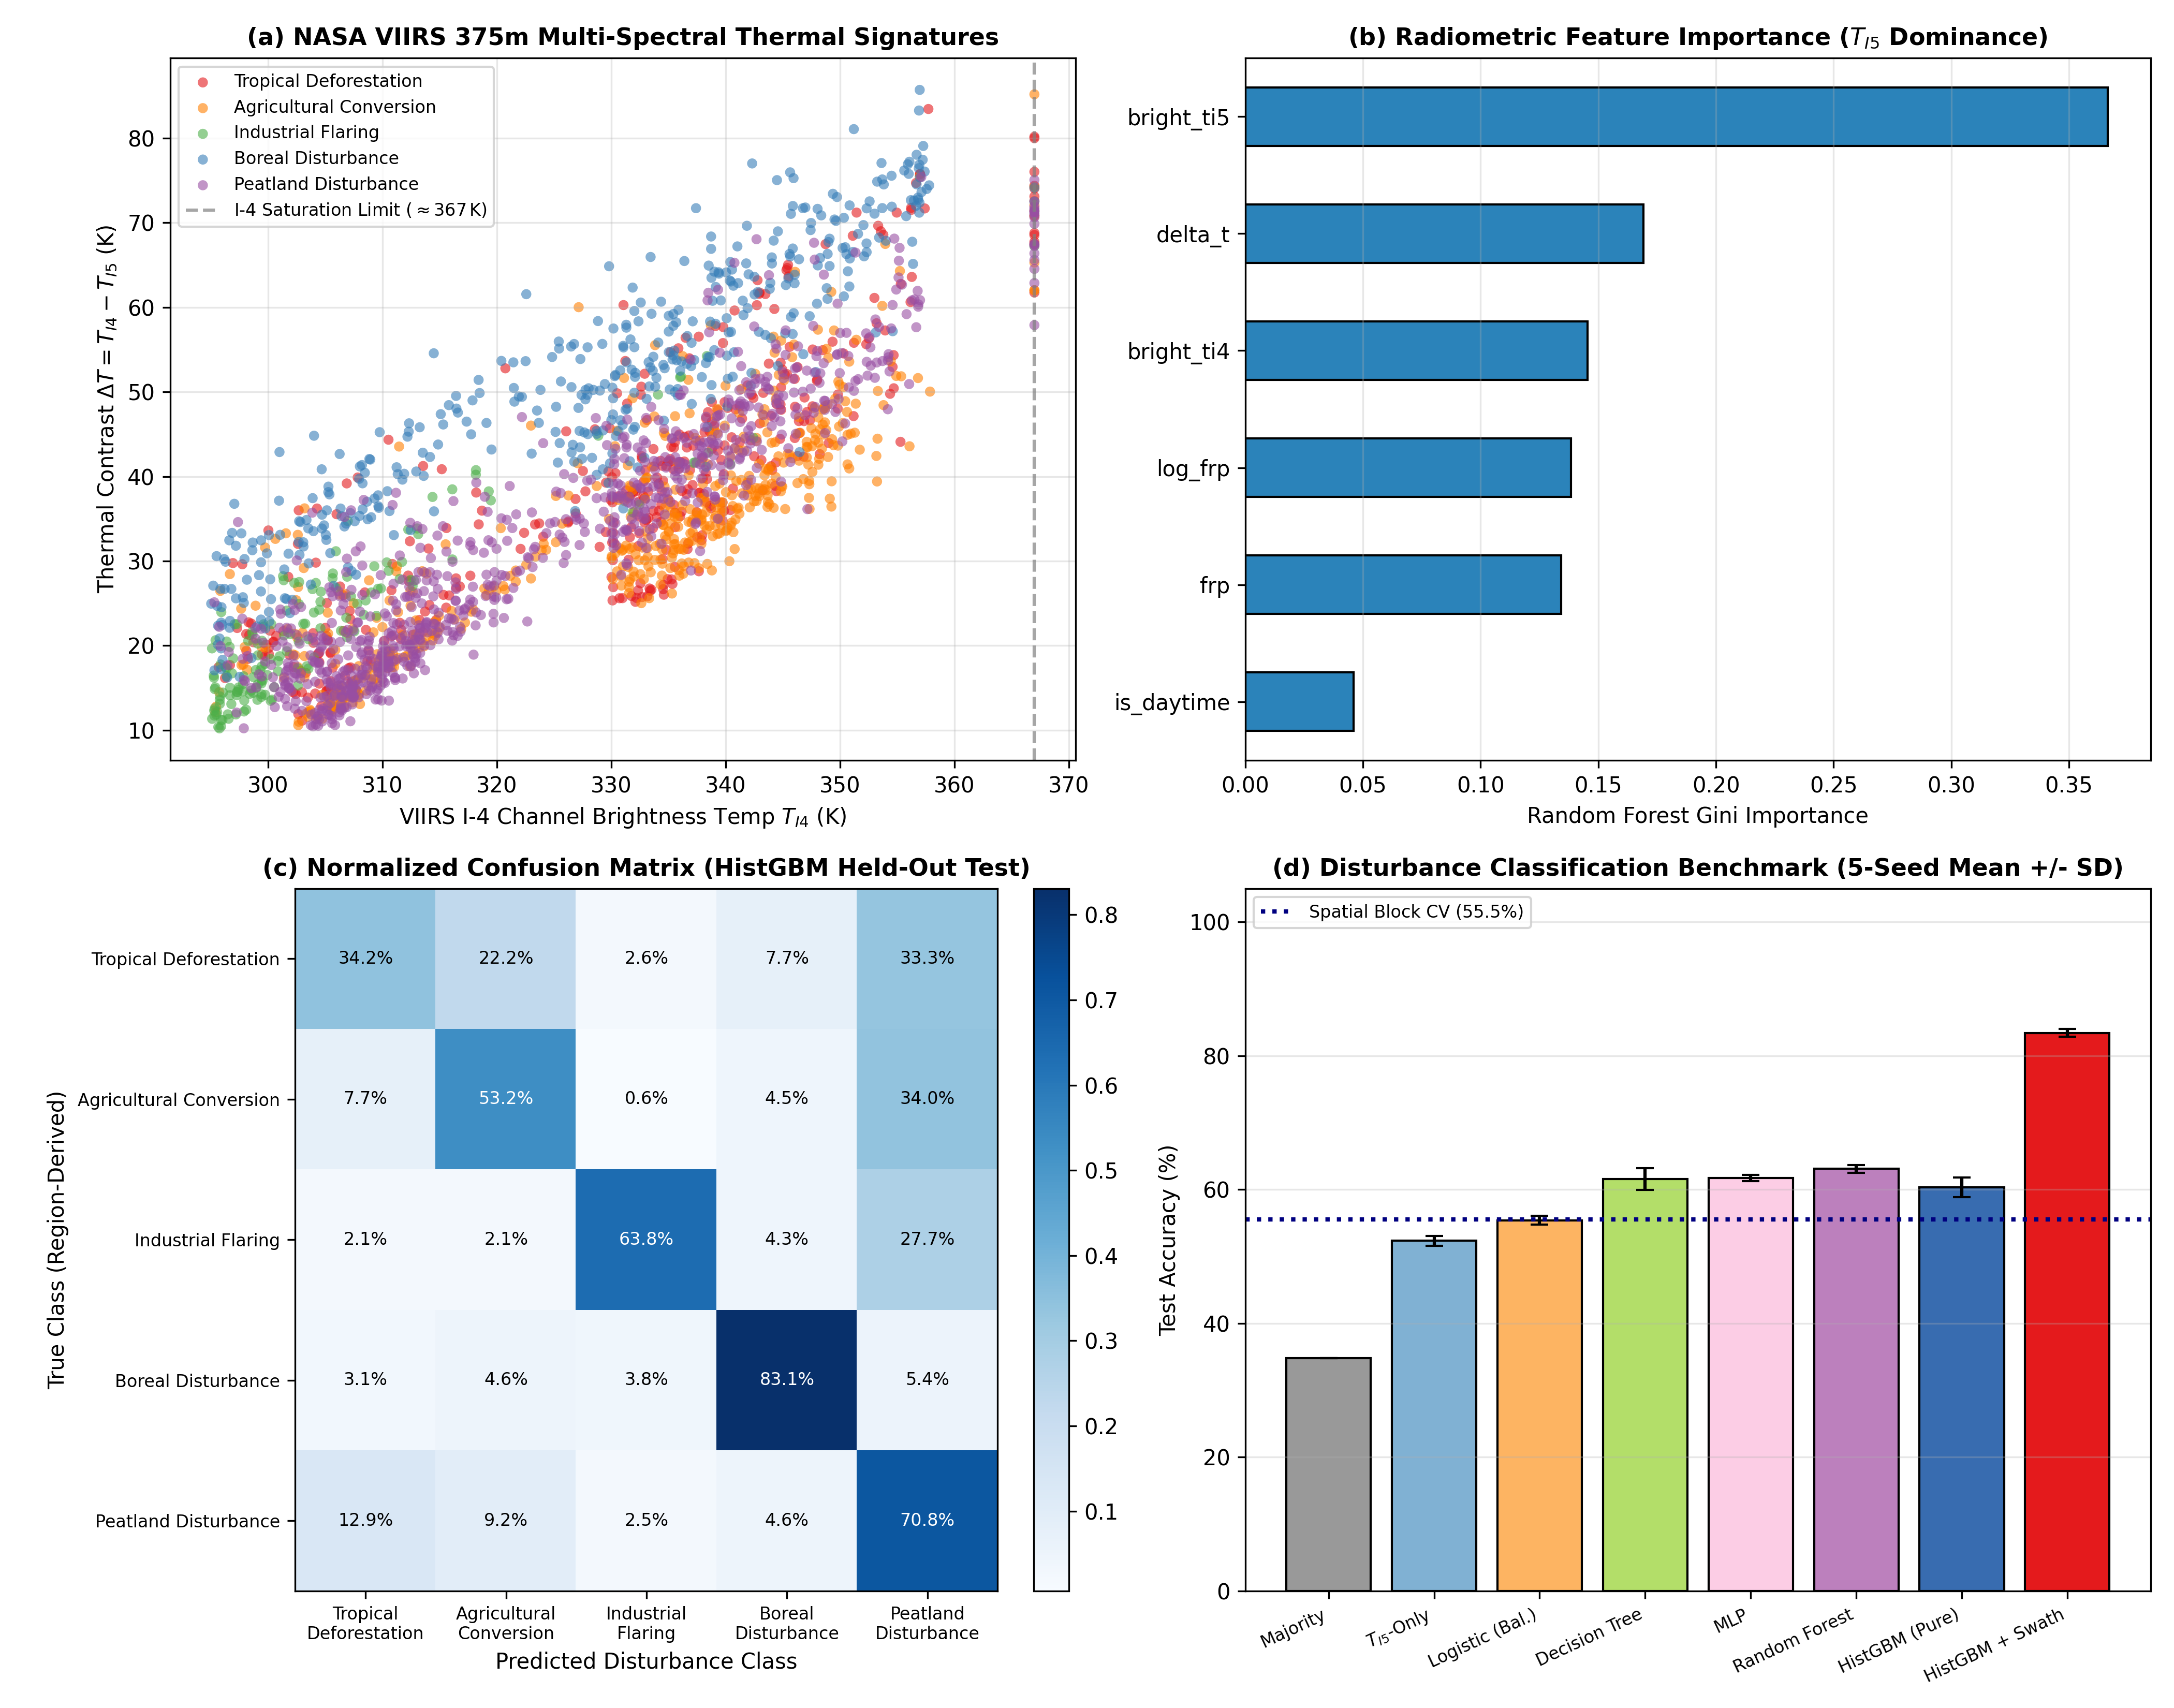
\includegraphics[width=0.95\textwidth]{figures/fig1_landuse_disturbance_benchmark.png}
\caption{Empirical evaluation on \numDetections{} NASA VIIRS 375m active satellite observations across five global disturbance regimes. (a) Multi-spectral thermal contrast signature: I-4 brightness temperature ($T_{I4}$) versus differential thermal contrast ($\Delta T = T_{I4} - T_{I5}$), highlighting sensor saturation at $367\,$K. (b) Random Forest Gini feature importances. (c) Normalized confusion matrix on held-out test detections for Histogram Gradient Boosting. (d) Disturbance classification benchmark across 8 model configurations (5-seed mean $\pm$ SD) alongside spatial block cross-validation.}
\label{fig:satellite_overview}
\end{figure*}

\section{Related Work}
\label{sec:related}

\subsection{Spaceborne Active Fire Radiometry and Thermal Anomaly Products}
Operational monitoring of terrestrial thermal anomalies relies on satellite radiometry in the mid-infrared (MIR, $\approx 3.9\,\mu\text{m}$) and thermal-infrared (TIR, $\approx 11\,\mu\text{m}$) spectral windows~\cite{schroeder2014}. The MODIS active fire product (MOD14)~\cite{giglio2016} established a multi-decade baseline at 1\,km nominal resolution, utilizing contextual potential fire pixel thresholding and Fire Radiative Power (FRP) quantification based on the Stefan-Boltzmann formulation~\cite{wooster2005}. The Visible Infrared Imaging Radiometer Suite (VIIRS) aboard Suomi-NPP enhanced spatial resolution to 375\,m in the I-band channels (I-4 at $3.74\,\mu\text{m}$ and I-5 at $11.45\,\mu\text{m}$), substantially improving the detection of sub-canopy and low-intensity fires while preserving swath coverage~\cite{schroeder2014}. Concurrently, specialized algorithms such as VIIRS Nightfire~\cite{elvidg2016} have mapped industrial petrochemical gas flaring using shortwave and midwave infrared radiances.

\subsection{Disturbance Regime Characterization and Driver Attribution}
While active fire algorithms detect the presence of thermal anomalies, characterizing the underlying land-use driver---distinguishing agricultural clearing from timber harvesting, industrial extraction, and natural wildfire---has traditionally relied on multi-year optical surface reflectance composites. Hansen et al.~\cite{hansen2013} mapped global forest cover loss extent at 30\,m resolution, while Curtis et al.~\cite{curtis2018} attributed dominant 10\,km drivers into commodity-driven deforestation, shifting agriculture, forestry, wildfire, and urbanization. Tyukavina et al.~\cite{tyukavina2022} and Morton et al.~\cite{morton2006} highlighted the distinct temporal dynamics of agricultural conversion in South America and peatland drainage fires in Southeast Asia~\cite{page2002}. However, optical forest-change products exhibit significant latency (often released annually), necessitating near-real-time thermal classification frameworks capable of rapid disturbance attribution.

\subsection{Sensor Swath Footprint Shortcuts and Geometric Artifact Mitigation}
A pervasive challenge in applying machine learning to raw satellite swath data is the influence of scan-angle geometry. In polar-orbiting cross-track scanners like VIIRS and MODIS, optical pixel footprint dimensions expand significantly from nadir toward the scan edge (the bow-tie effect)~\cite{wolfe2002}. When along-scan and along-track footprint dimensions are provided as predictive features, machine learning models can exploit spurious shortcut learning~\cite{geirhos2020} (associating specific scan angles with regional overpass orbits) rather than genuine combustion physics. Deliberately excluding geometric footprint parameters isolates pure radiometric attributes ($T_{I4}, T_{I5}, \Delta T, \text{FRP}$) and provides a generalizable baseline for multi-class disturbance characterization. Table~\ref{tab:literature_comparison} synthesizes prior remote sensing disturbance paradigms against the benchmark presented here.

\begin{table*}[t]
\caption{Comparison of Satellite Disturbance Characterization and Active Fire Attribution Frameworks}
\label{tab:literature_comparison}
\centering
\resizebox{\textwidth}{!}{%
\begin{tabular}{p{3.5cm}p{2.8cm}p{2.8cm}p{2.8cm}p{4.2cm}}
\toprule
\textbf{Framework / Sensor Product} & \textbf{Spatial Resolution} & \textbf{Primary Input Modality} & \textbf{Target Disturbance Class} & \textbf{Primary Methodological Limitation} \\
\midrule
Optical Global Forest Loss~\cite{hansen2013,curtis2018} & $30\text{ m}$ Landsat & Annual multi-spectral surface reflectance & Stand-replacement disturbance & Annual latency; misses sub-canopy and rapid burning \\
MODIS Active Fire (MOD14)~\cite{giglio2016} & $1\text{ km}$ nominal & Mid-infrared 4\,$\mu$m and 11\,$\mu$m channels & Coarse active fire detection & Pixel blurring ($1\text{ km}$); misses small clearings \\
VIIRS Nightfire Gas Flaring~\cite{elvidg2016} & $750\text{ m}$ M-band & Nighttime shortwave infrared (SWIR) & Industrial petrochemical flaring & Restricted to nighttime; vegetation fires excluded \\
Geometry-Conditioned Ablation & $375\text{ m}$ VIIRS & Swath footprints (\texttt{scan}, \texttt{track}) + radiances & Multi-class disturbance & Inflates accuracy by \shortcutBoost{} percentage points via orbital scan-angle shortcuts \\
\midrule
\textbf{Pure Radiometric Benchmark (This Work)} & \textbf{$375\text{ m}$ VIIRS I-Band} & \textbf{Thermal contrast ($\Delta T, T_{I4}, T_{I5}, \text{FRP}$)} & \textbf{5 Global Disturbance Biomes} & \textbf{Random pixel split (optimistic); single region per class; background $T_{I5}$ climate confounding} \\
\bottomrule
\end{tabular}%
}
\end{table*}


\section{NASA Satellite Observations and Feature Formulation}
\subsection{NASA FIRMS VIIRS 375m Active Sensor Records}
Data are acquired directly via the NASA Fire Information for Resource Management System (FIRMS) API for the VIIRS sensor aboard the Suomi National Polar-orbiting Partnership (Suomi-NPP) spacecraft, covering the acquisition window from \dateMin{} to \dateMax{}. The 375m I-band channels offer superior spatial resolution and thermal sensitivity for detecting fine-scale combustion and land-clearing anomalies compared to legacy 1~km MODIS products~\cite{giglio2016}.

Five contrasting global disturbance regimes were sampled:
\begin{enumerate}
    \item \textbf{Tropical Deforestation} (Brazilian Amazon, Mato Grosso and Rond\^{o}nia): Active clearing of primary tropical evergreen broadleaf forest along the deforestation frontier.
    \item \textbf{Agricultural Conversion} (Brazilian Cerrado, Maranh\~{a}o and Tocantins): Large-scale savanna conversion and crop residue burning.
    \item \textbf{Industrial Flaring} (Texas Permian Basin): Petrochemical extraction sites and flare stacks exhibiting persistent, high-temperature thermal anomalies.
    \item \textbf{Boreal Disturbance} (North American Boreal, Alberta and Northwest Territories): Coniferous taiga wildfire and forestry disturbance.
    \item \textbf{Peatland Disturbance} (Sumatra, Indonesia): Drained tropical peat swamp clearing with smoldering subterranean combustion.
\end{enumerate}
Across all five domains, $N = \numDetections{}$ satellite detections were ingested. Detections were partitioned into \numSpatialTiles{} spatial tiles of dimension 0.25$^\circ \times 0.25^\circ$ ($\approx 28\text{ km}$) for spatial validation. Exactly \numSaturatedPixels{} detections reach the operational sensor saturation ceiling ($T_{I4} \ge 367\text{ K}$).

\subsection{Physical Sensor Feature Space and Bi-Spectral Radiance Formulation}
\label{sec:dozier}
Following the classical Dozier sub-pixel radiance formulation~\cite{dozier1981,wooster2005,schroeder2014}, the spectral radiance $L(\lambda)$ observed by a satellite pixel containing a sub-pixel fire occupying fractional area $p \in (0, 1]$ at temperature $T_f$, surrounded by background surface at temperature $T_b$, is governed by Planck's law $B(\lambda, T)$:
\begin{equation}
L(\lambda) = p \cdot B(\lambda, T_f) + (1 - p) \cdot B(\lambda, T_b)
\end{equation}
Because Planck radiance increases exponentially faster with temperature at shorter wavelengths ($3.74\,\mu\text{m}$ for I-4 vs.\ $11.45\,\mu\text{m}$ for I-5), high-temperature flaming combustion sharply elevates $T_{I4}$ while barely perturbing $T_{I5}$, theoretically producing substantial thermal contrast ($\Delta T = T_{I4} - T_{I5}$). However, operational VIIRS I-4 channels saturate near $\approx 367\text{ K}$, and empirical active-fire detections reflect regional background conditions and sensor sampling constraints alongside flame properties. While explicit numerical inversion for $T_f$ and $p$ requires simultaneous non-linear multi-spectral solving with localized background estimates, the bi-spectral principle directly motivates our use of $\Delta T = T_{I4} - T_{I5}$ as an empirical physical feature capturing sub-pixel thermal intensity.

Our pure radiometric feature space extracts:
\begin{itemize}
    \item Mid-infrared 375m I-4 brightness temperature $T_{I4}$ (Kelvin).
    \item Thermal-infrared 375m I-5 brightness temperature $T_{I5}$ (Kelvin).
    \item Differential thermal contrast $\Delta T = T_{I4} - T_{I5}$ (Kelvin).
    \item Fire Radiative Power $\text{FRP}$ (MW) and log-transformed $\ln(1 + \text{FRP})$.
    \item Binary day/night solar illumination indicator ($d \in \{0, 1\}$).
\end{itemize}

\section{Methodology and Experimental Setup}
We evaluate ten model configurations across two experimental protocols: a 5-seed random 70/30 stratified train/test split and a 5-fold spatial block cross-validation:
\begin{enumerate}
    \item \textbf{Majority Baseline}: Predicts the most frequent class in the training partition.
    \item \textbf{Coordinates-Only (Lat/Lon)}: Boosted tree classifier trained solely on latitude and longitude to quantify geographic memorization.
    \item \textbf{Geometry-Only (Scan/Track)}: Boosted tree classifier trained solely on along-scan and along-track pixel footprint dimensions.
    \item \textbf{$T_{I5}$-Only (Ambient Baseline)}: Decision tree trained solely on background brightness temperature $T_{I5}$ to isolate ambient climate predictive power.
    \item \textbf{Logistic Regression (Class-Balanced)}: Linear classifier with standard feature scaling and inverse class-prevalence weighting to address class imbalance.
    \item \textbf{Decision Tree Baseline}: Single decision tree constrained to maximum depth 6.
    \item \textbf{Multi-Layer Perceptron (MLP)}: Fully connected neural network with two hidden layers ($64 \times 32$ neurons) and ReLU activations.
    \item \textbf{Random Forest Classifier}: Ensemble of 150 randomized decision trees with maximum depth 10.
    \item \textbf{Histogram Gradient Boosting (HistGBM)}: Histogram-based boosted tree classifier (150 iterations, learning rate 0.08).
    \item \textbf{HistGBM + Swath Geometry}: HistGBM trained with the addition of along-scan and along-track footprint geometry to quantify shortcut inflation.
\end{enumerate}

To evaluate out-of-tile generalization and eliminate spatial autocorrelation leakage, we also perform 5-fold Spatial Block Cross-Validation using \texttt{GroupKFold} over \numSpatialTiles{} spatial tiles of 0.25$^\circ$ resolution.

\section{Empirical Results}

\begin{table}[t]
\centering
\caption{Disturbance Characterization Benchmark on NASA VIIRS Detections ($N = \numDetections{}$, 5-Seed Mean $\pm$ SD).}
\label{tab:satellite_benchmark}
\resizebox{\columnwidth}{!}{%
\begin{tabular}{lcccc}
\toprule
\textbf{Model / Configuration} & \textbf{Accuracy (\%)} & \textbf{Macro-F1 (\%)} & \textbf{Weighted-F1 (\%)} & \textbf{Macro-Recall (\%)} \\
\midrule
\multicolumn{5}{l}{\textit{Reference and Control Baselines}} \\
Majority Baseline & 34.8 $\pm$ 0.0 & 10.3 $\pm$ 0.0 & 18.0 $\pm$ 0.0 & 20.0 $\pm$ 0.0 \\
Coordinates-Only (Lat/Lon) & 99.8 $\pm$ 0.1 & 99.8 $\pm$ 0.1 & 99.8 $\pm$ 0.1 & 99.8 $\pm$ 0.1 \\
Geometry-Only (Scan/Track) & 53.0 $\pm$ 1.0 & 47.3 $\pm$ 1.9 & 51.8 $\pm$ 1.1 & 45.7 $\pm$ 1.5 \\
$T_{I5}$-Only (Ambient Temp) & 52.3 $\pm$ 0.7 & 39.9 $\pm$ 2.7 & 47.3 $\pm$ 1.2 & 42.7 $\pm$ 1.4 \\
\midrule
\multicolumn{5}{l}{\textit{Pure Radiometric Classifiers}} \\
Logistic Regression (Balanced) & 55.4 $\pm$ 0.7 & 54.4 $\pm$ 0.9 & 55.5 $\pm$ 0.5 & 59.7 $\pm$ 1.2 \\
Decision Tree (Depth 6) & 61.6 $\pm$ 1.6 & 57.0 $\pm$ 1.0 & 58.7 $\pm$ 0.7 & 57.7 $\pm$ 1.5 \\
Multi-Layer Perceptron (MLP) & 61.7 $\pm$ 0.5 & 57.8 $\pm$ 0.7 & 59.1 $\pm$ 0.3 & 59.4 $\pm$ 0.9 \\
Random Forest (150 trees) & 63.1 $\pm$ 0.6 & 60.4 $\pm$ 1.4 & 61.6 $\pm$ 0.6 & 59.8 $\pm$ 1.8 \\
HistGradientBoosting & 60.3 $\pm$ 1.5 & 58.5 $\pm$ 2.0 & 59.5 $\pm$ 1.5 & 58.2 $\pm$ 2.1 \\
\midrule
\multicolumn{5}{l}{\textit{Orbital Swath Geometry Shortcut Ablation}} \\
HistGBM + Swath (Scan/Track) & \textbf{83.4 $\pm$ 0.6} & \textbf{81.3 $\pm$ 0.8} & \textbf{83.3 $\pm$ 0.6} & \textbf{80.8 $\pm$ 1.1} \\
\midrule
Spatial Block 5-Fold CV (HistGBM) & 55.5 $\pm$ 5.8 & 53.7 $\pm$ 5.2 & --- & --- \\
\bottomrule
\end{tabular}%
}
\end{table}

\begin{table}[t]
\centering
\caption{Empirical Thermal Radiometry Distributions Across Disturbance Classes (Median [IQR]).}
\label{tab:physical_distributions}
\resizebox{\columnwidth}{!}{%
\begin{tabular}{lccccc}
\toprule
\textbf{Disturbance Class} & $N$ & $T_{I4}$ (K) & $T_{I5}$ (K) & $\Delta T$ (K) & FRP (MW) \\
\midrule
Tropical Deforestation & 391 & 334.2 [27.8] & 292.3 [13.5] & 38.2 [21.0] & 6.05 [8.31] \\
Agricultural Conversion & 520 & 335.2 [30.5] & 297.5 [11.6] & 34.1 [17.4] & 4.04 [5.36] \\
Industrial Flaring & 157 & 300.3 [10.0] & 282.5 [5.3] & 20.5 [12.4] & 0.85 [0.71] \\
Boreal Disturbance & 431 & 331.3 [33.5] & 277.9 [10.9] & 51.6 [23.3] & 5.03 [12.29] \\
Peatland Disturbance & 800 & 318.9 [30.0] & 292.4 [7.6] & 30.0 [24.7] & 3.05 [4.61] \\
\bottomrule
\end{tabular}%
}
\end{table}


As detailed in Table~\ref{tab:satellite_benchmark}, Table~\ref{tab:physical_distributions}, and Fig.~\ref{fig:satellite_overview}:
\begin{itemize}
    \item \textbf{RQ1: Radiometric Discrimination and Shortcut Inflation}: Pure radiometric classifiers achieve \accRf{}\% accuracy (Random Forest) and \accHgb{}\% (HistGBM) on the held-out test cohort across 5 random seeds. When along-scan and along-track swath footprint parameters are added, accuracy surges to \accSwathGeom{}\% (a $+\shortcutBoost{}$ percentage point shortcut boost), reflecting a coupled interaction between sensor view geometry, footprint enlargement, and radiance (geometry alone yields \accGeomOnly{}\% accuracy, and radiometry alone yields \accHgb{}\%, while combined they reach \accSwathGeom{}\%). When evaluated under 5-fold Spatial Block Cross-Validation across \numSpatialTiles{} spatial tiles, pure radiometric accuracy drops to \accSpatialBlockCv{}$\pm$\accSpatialBlockCvStd{}\%, demonstrating that random pixel splitting inflates apparent test accuracy by \spatialLeakageInflation{} percentage points due to spatial autocorrelation. Coordinates-only classification achieves \accCoords{}\% accuracy, confirming that coordinates separate regional study areas with near-perfect fidelity.
    \item \textbf{RQ2: Non-Linear Ensembles vs.\ Balanced Linear Models}: The balanced Logistic Regression baseline achieves \accLogReg{}\% accuracy and \fOneLogReg{}\% macro-F1, trailing tree ensembles (\accRf{}\% and \accHgb{}\%) by $5$--$8$ percentage points. This performance gap demonstrates that non-linear feature interactions between background temperature $T_{I5}$ and sub-pixel thermal contrast $\Delta T$ substantially improve regime separation over linear combinations, even when class imbalance is explicitly countered with inverse frequency weighting.
    \item \textbf{RQ3: Physical Distributions across Biomes}: Table~\ref{tab:physical_distributions} details the empirical distributions of radiometry across biomes. Industrial flaring exhibits the lowest median $\Delta T$ (\flaringDeltaTMed{} K) and lowest median FRP (\flaringFrpMed{} MW). Because small flare tips within 375m pixels dissipate heat across the non-combusting background, flaring does not produce large pixel-averaged thermal contrasts in standard active fire products, resulting in $27.7\%$ misclassification into peatland smoldering. Conversely, Boreal wildfire exhibits the highest median thermal contrast ($\Delta T = \borealDeltaTMed{}\text{ K}$), driven by the cold sub-arctic background ($T_{I5} = \borealTiFiveMed{}\text{ K}$) rather than hotter flaming temperatures. Feature importance analysis (Fig.~\ref{fig:satellite_overview}(b)) confirms that background temperature $T_{I5}$ accounts for \featImpTiFive{}\% of Gini importance.
\end{itemize}

\section{Limitations}
\label{sec:limitations}
Several limitations should be considered when interpreting these findings:
\begin{enumerate}
    \item \textbf{Geographic Confounding of Disturbance Classes}: The five disturbance regimes are sampled from distinct geographic regions (Amazon, Cerrado, Permian Basin, Boreal taiga, and Sumatra). Consequently, the dominant feature ($T_{I5}$) reflects ambient regional surface temperature differences across biomes as well as combustion characteristics.
    \item \textbf{Spatial Autocorrelation and Evaluation Leakage}: Standard random pixel partitions allow adjacent pixels from the same fire front or satellite overpass to land in both training and test sets. Spatial block cross-validation demonstrates that true out-of-tile generalization accuracy is \accSpatialBlockCv{}$\pm$\accSpatialBlockCvStd{}\%.
    \item \textbf{Sensor Saturation Artifacts}: Operational VIIRS I-4 channels saturate near $\approx 367\text{ K}$, creating an artificial upper threshold in observed brightness temperatures for intense flaming combustion (\numSaturatedPixels{} pixels).
    \item \textbf{Snapshot vs.\ Temporal Evolution}: The model operates on instantaneous satellite detections from a 5-day window (\dateMin{} to \dateMax{}) rather than multi-temporal time series, precluding observation of post-fire vegetation recovery.
    \item \textbf{Regional Bounding-Box Labeling}: Disturbance labels are assigned based on established geographic bounding boxes for known disturbance frontiers rather than exhaustive parcel-by-parcel ground validation.
\end{enumerate}

\section{Data Availability}
\label{sec:data_availability}
Spaceborne active fire and thermal anomaly observations are openly distributed by NASA Land, Atmosphere Near real-time Capability for EOS (LANCE) Fire Information for Resource Management System (FIRMS) via the VIIRS 375m active fire product (VNP14IMGTDL / VJ114IMGTDL) at \url{https://firms.modaps.eosdis.nasa.gov/}. Land cover classification granules and biome boundaries are provided by the NASA USGS LP DAAC MODIS Terra+Aqua Combined Land Cover Type product (MCD12Q1 Version 6.1) accessible via Earthdata Search at \url{https://search.earthdata.nasa.gov/}. All spatial block partitioning scripts and benchmark evaluation code are available in the project repository (\url{https://github.com/CaceresCristhian/Satellite_LandUse}).

\section{Conclusion}
By evaluating \numDetections{} NASA VIIRS 375m active satellite sensor detections across five biomes, this work establishes an empirical benchmark for environmental disturbance characterization. We demonstrate that pure multi-spectral active-fire radiometry achieves \accRf{}\% test accuracy under random splits and \accSpatialBlockCv{}$\pm$\accSpatialBlockCvStd{}\% under spatial block cross-validation, while showing that incorporating orbital swath geometry boosts accuracy by \shortcutBoost{} percentage points through coupled swath geometry and radiometric interactions. Furthermore, physical distribution analysis reveals that background ambient temperature ($T_{I5}$) serves as a primary regional discriminator across global biomes, explaining the physical boundaries of satellite active-fire attribution.

\bibliographystyle{IEEEtran}
\bibliography{references}

\end{document}
